\section{Introduction To The Problem}
The Minimum Height Problem an optimization problem relating to ladder lotteries.
Let the \emph{height} of a ladder be the number of rows that a ladder has. 
The Minimum Height Problem asks, given $OptL\{\pi\}$, what ladders in the set with have the shortest height? 
Let $MinL\{\pi\} \subseteq OptL\{\pi\}$ such that the ladders in $MinL\{\pi\}$ are the shortest ladders from 
$OptL\{\pi\}$. Let \emph{a minimal ladder} be a ladder from $MinL\{\pi\}$. Given a permutation $\pi$, is there an algorithm for generating a minimal ladder
from $MinL\{\pi\}$? Let  Some tangential questions that result from this problem are the following. Let $MinL\{\pi_{N}\}$ 
be the set of all $MinL\{\pi\}$ for each permutation of order $N$. Recall that $OptL\{\pi_{N}\}$ is the set of all 
$OptL\{\pi\}$ of order $N$. Thus, $MinL\{\pi_{N}\} \subseteq OptL\{\pi_{N}\}$.  Firstly, 
is there an upper and lower bound for the heights of the ladder(s) in each $MinL\{\pi_{N}\}$? 
Secondly, what permutations of order $N$ result in ladders with a height of zero or one? 
Thirdly, is $|MinL\{\pi\}|=1$, or in other words is there 
only one ladder from $OptL\{\pi\}$ with a minimal height?\par 
Firstly I will address the tangential questions in the introduction. Following the tangential questions, 
I will provide a heuristic algorithm for generating one ladder from $MinL\{\pi\}$ in the procedures section. 
In the results section I will provide a table with the results of heuristic algorithm in comparison to the ladders 
in $MinL\{\pi\}$. Finally, in the analysis section there will be a discussion 
about the efficacy of the heuristic algorithm along with some applications of the algorithm.\par 
\subsection{Upper and Lower Bounds of the heights of the Ladders in each $MinL\{\pi_{N}\}$}
In order to address the question as to what the upper and lower bounds for each $MinL\{\pi_{N}\}$ 
some points of clarification need to be addressed. It must be noted that each $MinL\{\pi_{N}\} \subseteq$ of each
corresponding $OptL\{\pi_{N}\}$. For example, let $N=4$, there are $24$ or $4!$ $OptL\{\pi\}$ in $OptL\{\pi_{4}\}$, which is to say 
each permutation of order $4$ has its own $OptL\{\pi\}$. Each $MinL\{\pi_{4}\}$ is a subset of one of the $24$
$OptL\{\pi_{4}\}$. We are going to determine what the upper and lower bounds for the heights of the ladders in $MinL\{\pi_{N}\}$ are;
not the upper and lower bounds for the heights of the ladders in $OptL\{\pi_{N}\}$. Although the lower bound for the 
height of a ladder in $MinL\{\pi_{N}\}$ will also be the lower bound for the height of a ladder in $OptL\{\pi_{N}\}$
seeing as the ladder from $MinL\{\pi_{N}\}$ that has the lower bound for its height will be the shortest ladder 
from all $OptL\{\pi_{N}\}$.
\begin{lemma}
    The lower bound for the height of a ladder $MinL\{\pi_{N}\}$ is zero
\end{lemma} 
\begin{proof}
    If $\pi_{N}$ is the sorted permutation of order $N$ then there are no 
    bars in its ladder. Recall that a bar swaps an adjacent inversion in $\pi$.
    Seeing as there are no adjacent inversions in the sorted permutation of 
    order $N$, then there are no bars that need to be added to its corresponding 
    ladder. Since a ladder with no bars requires no rows, then the lower 
    bound for the height of a ladder from $MinL{\pi_{N}}$ is zero. This is 
    the ladder belonging to $OptL\{\pi_{ID_{N}}\}$.
\end{proof}\par 
The upper bound for the heights of the ladders in $MinL\{\pi_{N}\}$ is more difficult to prove than the lower bound. 
The lower bound is unique seeing as there is only one ladder with zero bars, the ladder belonging to 
the sorted permutation. With the upper bound however, it has yet to be shown if there is an upper bound for 
$MinL\{\pi_{N}\}$. Before proving the upper bound for $MinL\{\pi_{N}\}$ it must be shown how to 
derive the ladder with minimal height from the root ladder of the reverse permutation of order $N$.
Once we have established how to derive the ladder with minimal height from the root ladder 
of the reverse permutation of order $N$, it will be relatively easy to prove the upper bound 
for $MinL\{\pi_{N}\}$.\par 
 Let $Degen_{\pi_{N}}$ be the reverse permutation of order 
 $N$. Let $MinL_{Degen_{\pi_{N}}}$ be a ladder with the shortest height for $Degen_{\pi_{N}}$.
 Let $R_{Degen}$ be the root ladder from $OptL_\{Degen_{\pi_{N}}\}$. Recall that the root ladder is the ladder such 
    that no bar of a lesser element has crossed the route of a greater element. $R_{degen}$ requires 
    $2(N-1)-1$ rows. The $Nth$ element requires $N-1$ rows seeing as each of the bars in its route cannot be on the same row as 
    any other bar in the same route. The route of the $Nth$ element spans from the first column to the $N-1th$ column.
    The $N-1th$ element requires $N-2$ bars. Seeing as the $N-1th$  element is directly to the right of the $Nth$ element 
    in $Degen_{\pi_{N}}$ and it requires $N-2$ bars in $R_{Degen}$; its firt bar in $R_{Degen}$ will be in the first column and its last bar will be in the
    $N-2th$ column. Since the endpoints of no two bars can be touching, the last bar of the $N-1th$ route 
    will be one row below the last bar of the $Nth$ route. The same pattern applies to the $N-2th$ element in relation 
    to the $N-1th$ element and so on. Since all the bars of a lesser route in $R_{Degen}$ must be below the route of 
    any greater element, this means the first bar of any route will begin at column one in the ladder. Since each bar 
    of the $N-Kth$, $0 \leq K < (N-1)$, element requires $N-K-1$ bars in its route, the route will span from column one to 
    column $N-K-1$; each bar of the route cannot share a row with any other bar in the route.
   Yet since the last bar of the previous element's route is at the currently lowest row in the ladder, a new row 
   will need to be added to the ladder to accomodate the last bar of the current element.\par 
   
   In order to create a ladder with minimal height from $OptL_\{Degen_{\pi_{N}}\}$, one simply needs to 
   take $R_{Degen}$ and modify it. In order to modify $R_{Degen}$ correctly, consider what happens when 
   the bars of lesser elements are swapped above the bars of greater elements. Of course, if this is done then 
   the ladder is no longer $R_{Degen}$. Nonetheless, when the $N-1th$ route is swapped above the $Nth$ route, 
   this frees up an extra row in the ladder for the $N-2th$ route. This is the row where the last bar of the $N-1th$ element resided
   before it was swapped above the $Nth$ route. Now, the first bar of the $N-1th$ route will begin in column $2$ and end at column $N-1$. 
   Furthermore, a new row will need to be added to the top of the ladder in order to accomodate the first bar of the $N-1th$ route. Now the route 
   of the $N-2th$ element can be raised up a row seeing as its last bar will still be in column $N-2$ and the row 
   that was previously occupied by the last bar of the $N-1th$ element will be free. Then the $N-3$ route can be swapped above 
   element $N$ and begin at column $4$ and span to column $N-1$. Since a new row was already added aboev route $N$ for element $N-1$
   and the first bar of element $N-1$ route began at column $2$, the first bar of element $N-3$ and go in the 
   same row as element $N-1$ seeing as the only other bar in this new row is at column 2. By  swapping 
   all the  $N-Jth$, $1 \leq J < (N-1)$ and $J=2K+1$, routes  above the route of the route of the $Nth$
   element in $R_{Degen}$, the ladder is reconfigured to have the minimal height. This height is $N$ because the 
   $Nth$ element still requires $N-1$ rows, and the $N-1th$ element will require a new row to be added above 
   the row of the first bar of the $Nth$ element to accomodate its first bar. Essentially, if $N$ is even, then 
   swap the route of each odd element in $R_{Degen}$ above route $N$ and keep the route of each even element below route $N$ 
   to create a ladder with $N$ rows. If $N$ is odd, then swap the route of each even element in $R_{Degen}$ above the 
   $Nth$ element and keep the route of eahc odd element below the route of $N$ to create a ladder with $N$ rows. Please refer 
   to figure --fig for an example of modifying $R_{5,4,3,2,1}$ to $MinL_{5,4,3,2,1}$.\pagebreak


   \begin{center}
        \begin{figure}[!htp]
            \begin{minipage}{.4\textwidth}
                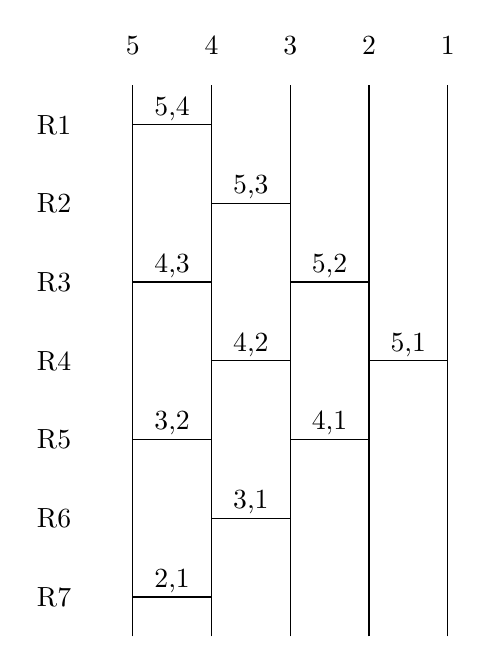
\begin{tikzpicture}
                    \draw(0, -1) to (0, 6);
                        %%draw the bars
                        \draw(0, 5.5) to (1, 5.5);
                            \node at (.5, 5.7){5,4};
                        \draw(0, 3.5) to (1, 3.5);
                            \node at (.5, 3.7){4,3};
                        \draw(0, 1.5) to (1, 1.5);
                            \node at (.5, 1.7){3,2};
                        \draw(0, -.5) to (1, -.5);
                            \node at (.5, -.3){2,1};
                    \draw(1, -1) to (1, 6);
                        \draw(1, 4.5) to (2, 4.5);
                            \node at(1.5, 4.7){5,3};
                        \draw(1, 2.5) to (2, 2.5);
                            \node at (1.5, 2.7){4,2};
                        \draw(1, .5) to (2, .5);
                            \node at(1.5, .7){3,1};
                    \draw(2, -1) to (2, 6);
                        \draw(2, 3.5) to (3, 3.5);
                            \node at(2.5, 3.7){5,2};
                        \draw(2, 1.5) to (3, 1.5);
                            \node at(2.5, 1.7){4,1};
                    \draw(3, -1) to (3, 6);
                        \draw(3, 2.5) to (4, 2.5);
                            \node at (3.5, 2.7){5,1};
                    \draw(4, -1) to (4, 6);

                    %%draw the rows
                    \node at (-1, 5.5){R1};
                    \node at(-1, 4.5){R2};
                    \node at(-1, 3.5){R3};
                    \node at (-1, 2.5){R4};
                    \node at(-1, 1.5){R5};
                    \node at (-1, 0.5){R6};
                    \node at (-1, -.5){R7};
                    %%draw the elements above the columns
                    \node at (0, 6.5){5};
                    \node at (1, 6.5){4};
                    \node at (2, 6.5){3};
                    \node at (3, 6.5){2};
                    \node at (4, 6.5){1};
                \end{tikzpicture}
            \end{minipage}
            \hfill
             \begin{minipage}{.4\textwidth}
                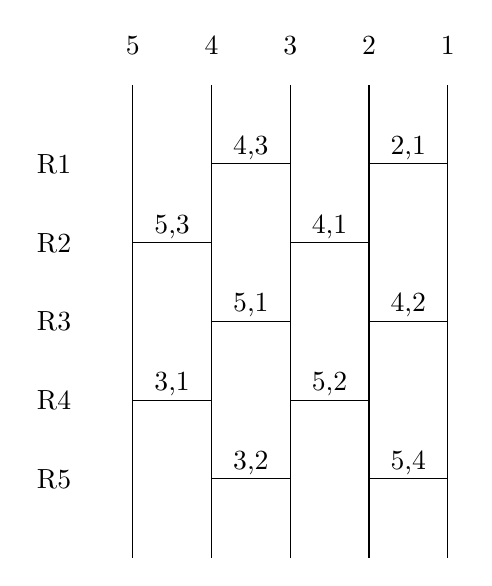
\begin{tikzpicture}
                    \draw(0, 0) to (0, 6);
                        \draw(0, 4) to (1, 4);
                            \node at(.5, 4.2){5,3};
                        \draw(0, 2) to (1, 2);
                            \node at(.5, 2.2){3,1};
                    \draw(1, 0) to (1, 6);
                        \draw(1, 3) to (2, 3);
                            \node at(1.5, 3.2){5,1};
                        \draw(1, 5) to (2, 5);
                            \node at(1.5, 5.2){4,3};
                        \draw(1, 1) to (2, 1);
                            \node at(1.5, 1.2){3,2};
                    \draw(2, 0) to (2, 6);
                        \draw(2, 2) to (3, 2);
                            \node at(2.5, 2.2){5,2};
                        \draw(2, 4) to (3, 4);
                            \node at(2.5, 4.2){4,1};
                    \draw(3, 0) to (3, 6);
                        \draw(3, 1) to (4, 1);
                            \node at(3.5, 1.2){5,4};
                        \draw(3, 3) to (4, 3);
                            \node at(3.5, 3.2){4,2};
                        \draw(3, 5) to (4, 5);
                            \node at(3.5, 5.2){2,1};
                    \draw(4, 0) to (4, 6);


                    %%nodes above
                    \node at (0, 6.5){5};
                    \node at (1, 6.5){4};
                    \node at (2, 6.5){3};
                    \node at (3, 6.5){2};
                    \node at (4, 6.5){1};

                    %%rows
                    \node at (-1, 5){R1};
                    \node at (-1, 4){R2};
                    \node at (-1, 3){R3};
                    \node at (-1, 2){R4};
                    \node at (-1, 1){R5};

                    %%nodes
    
                \end{tikzpicture}
            \end{minipage}
            \caption{The ladder to the left is $R_{5,4,3,2,1}$. The ladder to the left is $MinL_{5,4,3,2,1}$. Note that $N=5=2K+1$, thus 
            by swapping routes $2$ and $4$ above route $5$ whilst leaving route $3$ below route $5$ in $R_{5,4,3,2,1}$, we get 
            $MinL_{5,4,3,2,1}$. The height of $MinL_{5,4,3,2,1}$ is $5$. There is no way to reduce the height seeing as route $5$ still needs 
            $4$ rows and route $4$ needs one extra row for its first bar.}
        \end{figure}   

   \end{center}
   Now that $MinL_{Degen_{\pi_{N}}}$ has been established, we will go back to proving the upper bound for 
   $MinL\{\pi_{N}\}$. 
   \begin{lemma}
       The upper bound for $MinL\{\pi_{N}\}$ is $N$.
   \end{lemma}
   \begin{proof}
       We shall use a proof by contradiction. Suppose that the upper bound for the height of $MinL\{\pi_{N}\}$ was greater than $N$. (It cannot be less than $N$ because 
       we have already demonstrated that the minimal height of the ladder for the reverse permutation is $N$). Let $MinL_{Degen_{N}}$ be the 
       minimal ladder for the reverse permutation of order $N$. Refer to figure --fig for an example of $MinL_{5,4,3,2,1}$. It will be shown that for each 
       permutation of order $N$, one ladder from each permutation's corresponding $MinL\{\pi\}$ can be created by deriving it from $MinL_{Degen_{N}}$.
       Recall that a bar simply univerts an inversion in a permutation. By removing bars from $MinL_{Degen_{N}}$, that is effectively removing 
       inversions from $Degen_{\pi_{N}}$. Of course, when an inversion is removed from $Degen_{\pi_{N}}$, the resulting permutation 
       ceases to be the reverse permutation. Let $K$ be the number of bars in the current state of the ladder, wth $MinL_{Degen_{N}}$, $K=(N(N-1))/2$. Fpr each subsequent 
       ladder, $0 \leq K < (N(N-1))/2$. Thus, to create a ladder with minimal height for each permutation with $N-1$ inversions, simply remove the correct bar(s) from $MinL_{Degen_{N}}$. 
       Once all the ladders of minimal heights for each permutation with $N-1$ inversions has been created, simply remove the correct bar from each of these ladders 
       to derive all minimal heigt ladders for each permutation with $N-2$ inversions. This process continues until one ladder from each $MinL\{\pi\}$ has 
       been genreated from each $OptL\{\pi\}$ of order $N$. Since bars are only being removed from the initial ladder which is $MinL_{Degen_{N}}$, no more rows 
       will be added to the ladder. Removing a bar does not necessarily remove a row, but removing a bar definitely does not add a row to the ladder. Earlier we stated that 
       the height of $MinL_{Degen_{N}}$ is $N$, and at the same time we stated that we could create a ladder with minimal height 
       for each permutation of order $N$ by deriving it from $MinL_{Degen_{N}}$ by removing bars. Yet at the beginning of the proof, 
       we supposed the upper bound was greater than $N$ which contradicts the claim that by removing bars from  
       $MinL_{Degen_{N}}$ the height of  $MinL_{Degen_{N}}$ will not increase. Thus, the upper bound for $MinL_\{\pi_{N}\}$ is $N$. 
       Please refer to figure --fig for each ladder with minimal height generated derived from $MinL_{4,3,2,1}$. 

   \end{proof}\pagebreak

   \begin{center}
        \begin{figure}[!htp]
            %%L1
            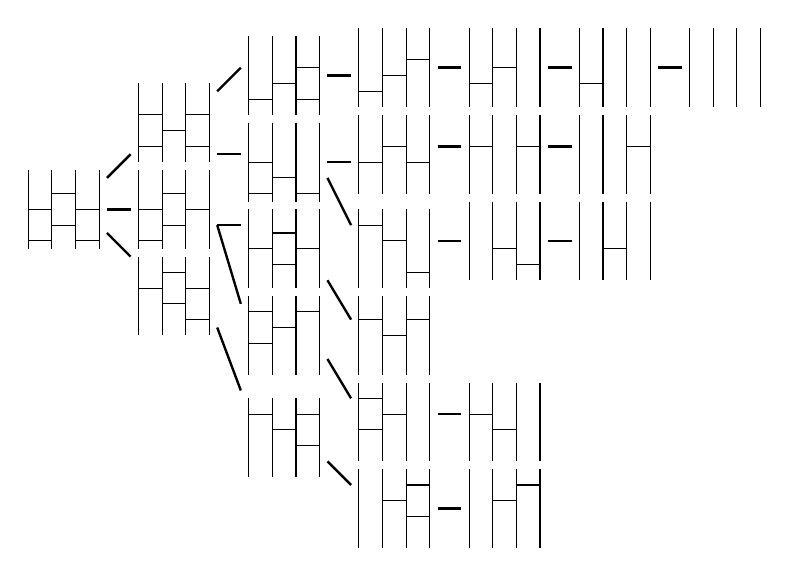
\begin{tikzpicture}
                \draw(0, -50) to (0, -51);
                    \draw(0, -50.5) to (.3, -50.5);
                    \draw(0, -50.9) to (.3, -50.9);
                \draw(0.3, -50) to (0.3, -51);
                    \draw(.3, -50.3) to (.6, -50.3);
                    \draw(.3, -50.7) to (.6, -50.7);
                \draw(0.6, -50) to (0.6, -51);
                    \draw(.6, -50.5) to (.9, -50.5);
                    \draw(.6, -50.9) to (.9, -50.9);
                \draw(0.9, -50) to (0.9, -51);
                
                \draw[line width = .3mm](1, -50.1) to (1.3, -49.8);
                \draw[line width = .3mm](1, -50.5) to (1.3, -50.5);
                \draw[line width = .3mm](1, -50.8) to (1.3, -51.1);
            
            %%L2
            \draw(1.4, -49.9) to (1.4, -48.9);
                \draw(1.4, -49.7) to (1.7, -49.7);
                \draw(1.4, -49.3) to (1.7, -49.3);
            \draw(1.7, -49.9) to (1.7, -48.9);
                \draw(1.7, -49.5) to (2, -49.5);
            \draw(2, -49.9) to (2, -48.9);
                \draw(2, -49.7) to (2.3, -49.7);
                \draw(2, -49.3) to (2.3, -49.3);
            
            \draw(2.3, -49.9) to (2.3, -48.9);
            %%L3
            \draw(1.4, -50) to (1.4, -51);
                \draw(1.4, -50.5) to (1.7, -50.5);
                \draw(1.4, -50.9) to (1.7, -50.9);
            \draw(1.7, -50) to (1.7, -51);
                \draw(1.7, -50.3) to (2, -50.3);
                \draw(1.7, -50.7) to (2, -50.7);
            \draw(2, -50) to (2, -51);
                \draw(2, -50.5) to (2.3, -50.5);
            \draw(2.3, -50) to (2.3, -51);

            %%L4
            \draw(1.4, -51.1) to (1.4, -52.1);
                \draw(1.4, -51.5) to (1.7, -51.5);
            \draw(1.7, -51.1) to (1.7, -52.1);
                \draw(1.7, -51.3) to (2, -51.3);
                \draw(1.7, -51.7) to (2, -51.7);
            \draw(2, -51.1) to (2, -52.1);
                \draw(2, -51.5) to (2.3, -51.5);
                \draw(2, -51.9) to (2.3, -51.9);
            \draw(2.3, -51.1) to (2.3, -52.1);

            \draw[line width=.3mm](2.4, -49) to (2.7, -48.7);
            \draw[line width=.3mm](2.4,-49.8) to (2.7, -49.8);
            \draw[line width=.3mm](2.4, -50.7) to (2.7, -50.7);
            \draw[line width=.3mm](2.4, -50.7) to (2.7, -51.7);
            \draw[line width = .3mm](2.4, -52) to (2.7, -52.8);

            %%L5
            \draw(2.8, -48.3) to (2.8, -49.3);
                \draw(2.8, -49.1) to (3.1, -49.1);
            \draw(3.1, -48.3) to (3.1, -49.3);
                \draw(3.1, -48.9) to (3.4, -48.9);
            \draw(3.4, -48.3) to (3.4, -49.3);
                \draw(3.4, -48.7) to (3.7, -48.7);
                \draw(3.4, -49.1) to (3.7, -49.1);
            \draw(3.7, -48.3) to (3.7, -49.3);

            %%L6
            \draw(2.8, -49.4) to (2.8, -50.4);
                \draw(2.8, -49.9) to (3.1, -49.9);
                \draw(2.8, -50.3) to (3.1, -50.3);
            \draw(3.1, -49.4) to (3.1, -50.4);
                \draw(3.1, -50.1) to (3.4, -50.1);
            \draw(3.4, -49.4) to (3.4, -50.4);
                \draw(3.4, -50.3) to (3.7, -50.3);
            \draw(3.7, -49.4) to (3.7, -50.4);

            %%L7
            \draw(2.8, -50.5) to (2.8, -51.5);
                \draw(2.8, -51) to (3.1, -51);
            \draw(3.1, -50.5) to (3.1, -51.5);
                \draw(3.1, -50.8) to (3.4, -50.8);
                \draw(3.1, -51.2) to (3.4, -51.2);
            \draw(3.4, -50.5) to (3.4, -51.5);
                \draw(3.4, -51) to (3.7, -51);
            \draw(3.7, -50.5) to (3.7, -51.5);
            %%L8
            \draw(2.8, -51.6) to (2.8, -52.6);
                \draw(2.8, -51.8) to (3.1, -51.8);
            \draw(3.1, -51.6) to (3.1, -52.6);
                \draw(3.1, -52) to (3.4, -52);
            \draw(3.4, -51.6) to (3.4, -52.6);
                \draw(3.4, -51.8) to (3.7, -51.8);
                \draw(2.8, -52.2) to (3.1, -52.2);
            \draw(3.7, -51.6) to (3.7, -52.6);
            
            %%L9
            \draw(2.8, -52.9) to (2.8, -53.9);
                \draw(2.8, -53.1) to (3.1, -53.1); 
            \draw(3.1, -52.9) to (3.1, -53.9);
                \draw(3.1, -53.3) to (3.4, -53.3);
            \draw(3.4, -52.9) to (3.4, -53.9);
                \draw(3.4, -53.1)to(3.7, -53.1);
                \draw(3.4, -53.5) to (3.7, -53.5);
            \draw(3.7, -52.9) to (3.7, -53.9);
            %%Lines
            \draw[line width = .3mm](3.8,-48.8) to (4.1,-48.8);
            \draw[line width = .3mm](3.8,-49.9) to (4.1,-49.9);
            \draw[line width = .3mm](3.8, -50.1) to (4.1, -50.7);
            \draw[line width = .3mm](3.8, -51.4) to (4.1, -51.9);
            \draw[line width = .3mm](3.8,-52.4) to (4.1,-52.9);
            \draw[line width = .3mm](3.8,-53.7) to (4.1,-54);

            %%L10
            \draw(4.2, -48.2) to (4.2, -49.2);
                \draw(4.2, -49) to (4.5, -49);
            \draw(4.5, -48.2) to (4.5, -49.2);
                \draw(4.5, -48.8) to (4.8, -48.8);
            \draw(4.8, -48.2) to (4.8, -49.2);
                \draw(4.8, -48.6) to (5.1, -48.6);
            \draw(5.1, -48.2) to (5.1, -49.2);

            %%L11
            \draw(4.2, -49.3) to (4.2, -50.3);
                \draw(4.2, -49.9) to (4.5, -49.9);
            \draw(4.5, -49.3) to (4.5, -50.3);
                \draw(4.5, -49.7) to (4.8, -49.7);
            \draw(4.8, -49.3) to (4.8, -50.3);
                \draw(4.8, -49.9) to (5.1, -49.9);
            \draw(5.1, -49.3) to (5.1, -50.3);
             %%L12
             \draw(4.2, -49.3) to (4.2, -50.3);
                \draw(4.2, -49.9) to (4.5, -49.9);
            \draw(4.5, -49.3) to (4.5, -50.3);
                \draw(4.5, -49.7) to (4.8, -49.7);
            \draw(4.8, -49.3) to (4.8, -50.3);
                \draw(4.8, -49.9) to (5.1, -49.9);
            \draw(5.1, -49.3) to (5.1, -50.3);

            %%L12
            \draw(4.2, -50.5) to (4.2, -51.5);
                \draw(4.2, -50.7) to (4.5, -50.7);
            \draw(4.5, -50.5) to (4.5, -51.5);
                \draw(4.5, -50.9) to (4.8, -50.9);
            \draw(4.8, -50.5) to (4.8, -51.5);
                \draw(4.8, -51.3) to (5.1, -51.3);
            \draw(5.1, -50.5) to (5.1, -51.5);

            %%L13
            \draw(4.2, -51.6) to (4.2, -52.6);
                \draw(4.2, -51.9) to (4.5, -51.9);
            \draw(4.5, -51.6) to (4.5, -52.6);
                \draw(4.5, -52.1) to (4.8, -52.1);
            \draw(4.8, -51.6) to (4.8, -52.6);
                \draw(4.8, -51.9) to (5.1, -51.9);
            \draw(5.1, -51.6) to (5.1, -52.6);

            %%L14
            \draw(4.2, -52.7) to (4.2, -53.7);
                \draw(4.2, -52.9) to (4.5, -52.9);
                \draw(4.2, -53.3) to (4.5, -53.3);
            \draw(4.5, -52.7) to (4.5, -53.7);
                \draw(4.5, -53.1) to (4.8, -53.1);
            \draw(4.8, -52.7) to (4.8, -53.7);
            \draw(5.1, -52.7) to (5.1, -53.7);

            %%L15
             \draw(4.2, -53.8) to (4.2, -54.8);
            \draw(4.5, -53.8) to (4.5, -54.8);
                \draw(4.5, -54.2) to (4.8, -54.2);
            \draw(4.8, -53.8) to (4.8, -54.8);
                \draw(4.8, -54) to (5.1, -54);
                \draw(4.8, -54.4) to (5.1, -54.4);
            \draw(5.1, -53.8) to (5.1, -54.8);

            %%Lines
            \draw[line width = .3mm](5.2, -48.7) to (5.5, -48.7);
            \draw[line width = .3mm](5.2, -49.7) to (5.5, -49.7);
            \draw[line width = .3mm](5.2, -50.9) to (5.5, -50.9);
            \draw[line width = .3mm](5.2, -53.1) to (5.5, -53.1);
            \draw[line width = .3mm](5.2, -54.3) to (5.5, -54.3);

            %%Ladders
            %%l16
            \draw(5.6, -48.2) to (5.6, -49.2);
                \draw(5.6, -48.9) to (5.9, -48.9);
            \draw(5.9, -48.2) to (5.9,  -49.2);
                \draw(5.9, -48.7) to (6.2, -48.7);
            \draw(6.2, -48.2) to (6.2,  -49.2);
            \draw(6.5, -48.2) to (6.5,  -49.2);
            %%l17
            \draw(5.6, -49.3) to (5.6, -50.3);
                \draw(5.6, -49.7) to (5.9, -49.7);
            \draw(5.9, -49.3) to (5.9, -50.3);
            \draw(6.2, -49.3) to (6.2, -50.3);
                \draw(6.2, -49.7) to (6.5, -49.7);
           \draw(6.5, -49.3) to (6.5, -50.3);

            %%l18
            \draw(5.6, -50.4) to (5.6, -51.4);
            \draw(5.9, -50.4) to (5.9, -51.4);
                \draw(5.9, -51) to (6.2, -51);
            \draw(6.2, -50.4) to (6.2, -51.4);
                \draw(6.2, -51.2) to (6.5, -51.2);
            \draw(6.5, -50.4) to (6.5, -51.4);

            %%l19
            \draw(5.6, -52.7) to (5.6, -53.7);
                \draw(5.6, -53.1) to (5.9, -53.1);
            \draw(5.9, -52.7) to (5.9, -53.7);
                \draw(5.9, -53.3) to (6.2, -53.3);
            \draw(6.2, -52.7) to (6.2, -53.7);
            \draw(6.5, -52.7) to (6.5, -53.7);

            %l20
            \draw(5.6, -53.8) to (5.6, -54.8);
            \draw(5.9, -53.8) to (5.9, -54.8);
                \draw(5.9, -54.2) to (6.2, -54.2);
            \draw(6.2, -53.8) to (6.2, -54.8);
                \draw(6.2, -54) to (6.5, -54);
            \draw(6.5, -53.8) to (6.5,-54.8);

            %%Lines
            \draw[line width = .3mm](6.6, -48.7) to (6.9, -48.7);
            \draw[line width = .3mm](6.6, -49.7) to (6.9, -49.7);
            \draw[line width = .3mm](6.6, -50.9) to (6.9, -50.9);


             %%l21
            \draw(7, -48.2) to (7, -49.2);
                \draw(7, -48.9) to (7.3, -48.9);
            \draw(7.3, -48.2) to (7.3,  -49.2);
            \draw(7.6, -48.2) to (7.6,  -49.2);
            \draw(7.9, -48.2) to (7.9,  -49.2);
            %%l22
            \draw(7, -49.3) to (7, -50.3);
            \draw(7.3, -49.3) to (7.3, -50.3);
            \draw(7.6, -49.3) to (7.6, -50.3);
                \draw(7.6, -49.7) to (7.9, -49.7);
           \draw(7.9, -49.3) to (7.9, -50.3);

            %%l23
            \draw(7, -50.4) to (7, -51.4);
            \draw(7.3, -50.4) to (7.3, -51.4);
                \draw(7.3, -51) to (7.6, -51);
            \draw(7.6, -50.4) to (7.6, -51.4);
            \draw(7.9, -50.4) to (7.9, -51.4);

            \draw[line width = .3mm](8, -48.7) to (8.3, -48.7);
             \draw(8.4, -48.2) to (8.4, -49.2);
             \draw(8.7, -48.2) to (8.7, -49.2);
             \draw(9, -48.2) to (9, -49.2);
             \draw(9.3, -48.2) to (9.3, -49.2);
        \end{tikzpicture}
        \end{figure}
   \end{center}

   \subsection{Permutations of order $N$ resulting in ladders with minimal heights of zero or one}
   There are some permutations of order $N$ which result in ladders with a minimal height of zero or one.
   There is only one permutation of order $N$ which results in a minimal ladder with a height of zero, 
   namely the idendity permutation. This point has already been proven in the lemma for the lower bound of the 
   minimal height. What is more interesting is the permutations of order $N$ which result in ladders with 
   a minimal height of one. One may be tempted to assume that if the idendity permutation results in a minimal ladder 
   with a height of zero, then all ladders with exactly one permutation result in a minimal ladder with a height of one.
   Although this is true, it is only partially true. There are more permutations of order $N$ with more than one inversion 
   which result in minimal ladders with a height of one.